\documentclass{article}
\usepackage[italian]{babel}
\usepackage[utf8x]{inputenc}
\usepackage[T1]{fontenc}
\usepackage{graphicx}
\usepackage[colorinlistoftodos]{todonotes}
\usepackage[colorlinks=true, allcolors=tudelftblue]{hyperref} %sets hyperlink colour
\usepackage{caption}
\usepackage{subcaption}
\usepackage{xcolor}
\usepackage{roboto} % for Roboto Slab font
\usepackage{float}
\usepackage{titling} 
\usepackage{blindtext}\usepackage{titlesec}
\usepackage[square,sort,comma,numbers]{natbib}
\usepackage[colorinlistoftodos]{todonotes}
\usepackage{tikz}
\usepackage{geometry}
\usepackage{sectsty}
\usepackage{amsmath}
\usepackage{tikzpagenodes}
\usepackage{booktabs}
\usepackage{listings}
\usepackage{svg}

\usepackage[labelfont=bf, labelsep=colon]{caption}
\captionsetup[table]{name=Tabella, position=bottom}
\captionsetup[figure]{name=Schema, position=bottom}


\definecolor{tudelftdarkblue}{RGB}{0,0,0}
\definecolor{tudelftcyan}{RGB}{209,65,36}
\definecolor{tudelftblue}{RGB}{99, 102, 106}
\geometry{a4paper, margin=2cm}
\allsectionsfont{\color{black}} %sets colour for all headers
\usepackage{helvet}
\renewcommand{\familydefault}{\sfdefault}
\sectionfont{\fontfamily{RobotoSlab-TLF}\selectfont}
%%%%%%%%%%%%%%%%%%%%%%%%%%%%%%%%%%%%%%%%%%%%%%%%%%%%%%%%%
\begin{document}

\begin{titlepage}
    \fontfamily{RobotoSlab-TLF}\selectfont 
%%%%%%%%%%%%%%%%%%%%%%%%%%%%%%%%%%%%%%%%%%%%%%%%%%%%%%%%%%UNCOMMENT THE FOLLOWING FOR LESS "PLAIN" TITLE PAGE (SELECT WITH MOUSE AND PRESS CTRL AND /)

    % \begin{tikzpicture}[remember picture,overlay]
    %     % Set seed for random number generator
    %     \pgfmathsetseed{4}
    %     % Define the text area to avoid
    %     \path (current page text area.south west) rectangle (current page text area.north east);
    %     % Adding circles spread over the entire page
    %     \foreach \x in {1,...,1000}
    %         \draw[tudelftdarkblue] (current page.south west) ++(rand*\paperwidth,rand*\paperheight) circle (rand*0.3);
    %     % Define coordinates for the corners of the white box
    %     \coordinate (A) at ([shift={(-8cm,12cm)}]current page.center);
    %     \coordinate (B) at ([shift={(8cm,-5cm)}]current page.center);
    %     % Draw the white background box
    %     \fill[white] (A) rectangle (B);
    %     % Adding equations as background features
    %     \node[anchor=center,rotate=20,text=tudelftcyan] at ([shift={(-7cm,-2cm)}]current page.center) {\fontsize{18}{22}\selectfont
    %     $\nabla^2 T - \frac{1}{\alpha}\frac{\partial T}{\partial t} = 0$};
    %     \node[anchor=center,rotate=-15,text=tudelftcyan] at ([shift={(5cm,-4cm)}]current page.center) {\fontsize{18}{22}\selectfont
    %     $\frac{\partial \rho}{\partial t} + \nabla \cdot (\rho \mathbf{v}) = 0$};
    %     \node[anchor=center,rotate=20,text=tudelftcyan] at ([shift={(6cm,4cm)}]current page.center) {\fontsize{18}{22}\selectfont
    %     $a^2 + b^2 = c^2$};
    %     \node[anchor=center,rotate=10,text=tudelftcyan] at ([shift={(7cm,-2cm)}]current page.center) {\fontsize{18}{22}\selectfont
    %     $E = \frac{\sigma}{\varepsilon}$};
    %     \node[anchor=center,rotate=-10,text=tudelftcyan] at ([shift={(-6cm,4cm)}]current page.center) {\fontsize{18}{22}\selectfont
    %     $F = ma$};
    %     \node[anchor=center,rotate=5,text=tudelftcyan] at ([shift={(-4cm,-5cm)}]current page.center) {\fontsize{18}{22}\selectfont
    %     $Q = -\frac{kA}{\mu} \frac{\Delta P}{L}$};
    % \end{tikzpicture}
    
%%%%%%%%%%%%%%%%%%%%%%%%%%%%%%%%%%%%%%%%%%%%%%%%%%%%%%%%%%
    \vspace*{3cm}
    
    \centering
    {\Huge \textbf{\textcolor{black}{Progetto Basi di dati}}}\\[1.5cm]
    \textsc{\LARGE Corso di Informatica}\\[0.5cm]
    \text{\large MN1-525}\\[2cm]
    
    {\Large \textbf{\textcolor{tudelftdarkblue}{Autori:}}}\\[0.5cm]
    \begin{tabular}{c}
        \Large \textcolor{tudelftdarkblue}{Bilotti Alessandro (206409)}
        % \Large \textcolor{tudelftdarkblue}{Author 2 (1234567)} \\
        % \Large \textcolor{tudelftdarkblue}{Author 3 (9876543)} \\
    \end{tabular}\\[2cm]
    
    {\Large \textcolor{tudelftdarkblue}{\today}}
    
    \vfill
    \begin{center}
        
\includegraphics[width=0.6\textwidth]{images/Logo_C_Positivo_Colore.png}
    \end{center}
\end{titlepage}

%%% Create a table of contents
\tableofcontents
\newpage

\addcontentsline{toc}{section}{Introduzione}
\section*{Introduzione}
\textbf{Greenrail\cite{Greenrail}} è un'azienda italiana, riconosciuta a livello internazionale come attore innovativo del settore ferroviario e come esempio di sviluppo industriale sostenibile secondo i principi dell'economia circolare.

\noindent Greenrail realizza i propri prodotti con plastica e gomma riciclate. Le soluzioni proposte riducono vibrazioni e impatto ambientale, aumentano la durata delle infrastrutture e possono integrare tecnologie smart (es.\ sensori o pannelli solari).

\section{Definizione dei requisiti}

\subsection{Vista Cliente}
I clienti della base dati di Greenrail rappresentano la parte finale della catena di valore, comprendono aziende e enti del settore delle infrastrutture ferroviarie. Questi possono essere gestori pubblici o privati di linee ferroviarie, imprese edili operanti su appalto pubblico, o società di progettazione infrastrutturale. I clienti devono fornire i seguenti dati: ragione sociale, tipologia (gestore, appaltatore, progettista, etc.), indirizzo (Paese, città, via, CAP), recapiti (telefono, email), codice fiscale e/o partita IVA.\\

\noindent Dopo aver consultato il catalogo dei prodotti, i clienti hanno la possibillità di effettuare richieste d’ordine, scaricare schede tecniche delle traversine, specificare i requisiti di installazione (es.\ condizioni climatiche, peso supportato, durata stimata). Per ogni ordine viene creata una commessa contenente informazioni dettagliate sul tipo di traversina scelta (Standard, Solar, LinkBox), quantità, località di destinazione ed eventuali note operative.

\noindent Il sistema tiene traccia dell'intera relazione cliente-azienda: dalle richieste iniziali di preventivo alle commesse in lavorazione, fino alla fase post-installazione. Ogni cliente ha accesso allo storico ordini e può essere associato a uno o più tecnici o partner logistici.

\subsection{Vista Produttore}
Il produttore rappresenta il personale tecnico addetto alla realizzazione fisica delle traversine nei centri di produzione. Ogni produttore ha un identificativo univoco, nome, cognome, qualifica, turno di lavoro, impianto di assegnazione e salario.

\noindent Il sistema consente la tracciabilità delle attività di produzione: per ogni traversina, si registrano le specifiche (variano in base al modello), la data di produzione, i materiali utilizzati, il tecnico assegnato e il numero di serie delle traversine.

\noindent I produttori devono poter visualizzare le specifiche tecniche richieste per ogni commessa, inclusi eventuali vincoli o personalizzazioni richieste dal cliente.

\noindent È inoltre previsto un registro delle non conformità rilevate in fase di produzione.

\subsection{Vista Installatore}
L’installatore è il tecnico incaricato della posa in opera delle traversine lungo le tratte ferroviarie. Può coincidere con il produttore o essere una figura distinta. Ogni installatore ha un codice identificativo, nome, cognome, zona geografica di competenza, e calendario di interventi.\\

\noindent Per ogni attività di installazione, il sistema deve registrare: numedi di serie delle traversine, località di installazione, data e durrata dell'installazione. Le installazioni sono sempre collegate a una specifica commessa cliente e devono rispettare i requisiti previsti.

\noindent Il sistema deve permettere il monitoraggio degli interventi conclusi e programmati, e registrare note tecniche utili per valutazioni future.

\subsection{Vista Amministratore}
L’amministratore è una figura di gestione centrale, responsabile del coordinamento delle operazioni e delle relazioni tra clienti, produttori e installatori.\\

\noindent L'amministratore gestisce tutte le entità presenti: clienti, ordini, commesse, produzione e installazione.

\noindent L’amministratore può scrivere report su quantità prodotte/installate, sostenibilità dei materiali e conformità dei certificati.

\noindent Inoltre, può intervenire per modificare dati errati, chiudere commesse, o aggiornare il catalogo prodotti.

\section{Analisi e schema scheletro}
\subsection{Analisi requisiti e schema scheletro per il Cliente}

\begin{table}[H]
    \begin{tabular}{|l|l|l|l|}
    \hline
    \textbf{Termine} & Descrizione                                                                                                      & Sinonimi                                                & Collagamenti                                                                                                  \\ \hline
    Cliente          & \begin{tabular}[c]{@{}l@{}}Enti o aziende, pubblici o privati,\\ nel settore ferroviario\end{tabular}            & \begin{tabular}[c]{@{}l@{}}Azienda,\\ Ente\end{tabular} & Prodotto, Amministratore                                                                                      \\ \hline
    Amministratore   & Coordinatore generale                                                                                            & Manager                                                 & Cliente, Prodotto                                                                                             \\ \hline
    Prodotto         & Articolo venduto da Greenrail                                                                                    & Traversina                                              & \begin{tabular}[c]{@{}l@{}}Cliente, Amministratore,\\ Produttore, Installatore,\\ Certificazione\end{tabular} \\ \hline
    Produttore       & Soggetta che realizza il prodotto                                                                                & -                                                       & Prodotto                                                                                                      \\ \hline
    Installatore     & Soggetto che installa il prodotto                                                                                & -                                                       & Prodotto                                                                                                      \\ \hline
    Certificato      & \begin{tabular}[c]{@{}l@{}}Certificazione che attesta la\\ sostenibilità e sicurezza del\\ prodotto\end{tabular} & -                                                       & Prodotto                                                                                                      \\ \hline
    \end{tabular}
    \caption{Glossario dei concetti del Cliente}
\end{table}

\begin{figure}[H]
    \centering
    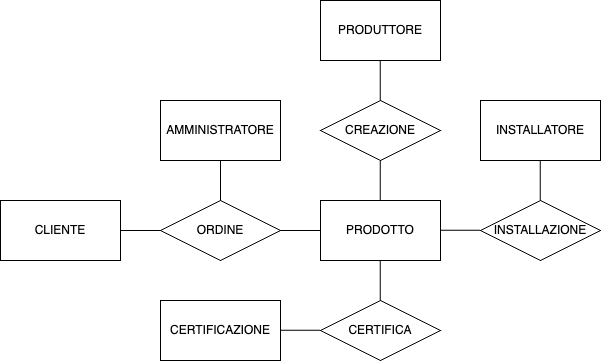
\includegraphics[width=12cm]{images/cliente.drawio.png}\\
    \caption{Schema scheletro della vista del Cliente}
\end{figure}

\subsection{Analisi requisiti e schema scheletro per il Produttore}

\begin{table}[H]
    \begin{tabular}{|l|l|l|l|}
    \hline
    \textbf{Termine} & Descrizione                                                                     & Sinonimi   & Collegamenti         \\ \hline
    Produttore       & Soggetto che realizza il prodotto                                               & -          & Sede                 \\ \hline
    Sede             & Luogo fisico                                                                    & Azienda    & Produttore           \\ \hline
    Team             & Insieme di produttori                                                           & Squadra    & Produttore, Prodotto \\ \hline
    Prodotto         & Articolo venduto da Greenrail                                                   & Traversina & Materiale, Team      \\ \hline
    Materiale        & \begin{tabular}[c]{@{}l@{}}Materiale di cui si compone un\\ prodotto\end{tabular} & -          & Fornitore, Prodotto  \\ \hline
    Fornitore        & Soggetto che fornisce materiale                                                 & -          & Materiale            \\ \hline
    \end{tabular}
    \caption{Glossario dei concetti del Produttore}
    \end{table}

\begin{figure}[H]
    \centering
    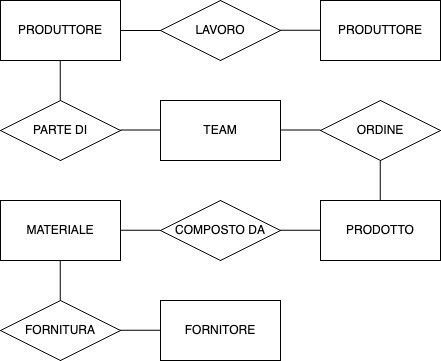
\includegraphics[width=10cm]{images/produttore.drawio.png}\\
    \caption{Schema scheletro della vista del Produttore}
\end{figure}

\subsection{Analisi requisiti e schema scheletro per l'Installatore}

\begin{table}[H]
    \begin{tabular}{|l|l|l|l|}
    \hline
    \textbf{Termine} & Descrizione                                                                                             & Sinonimi                                                 & Collegamenti                                                                 \\ \hline
    Installatore     & Soggetto che installa il prodotto                                                                       & -                                                        & Tratta, Prodotto                                                             \\ \hline
    Tratta           & Luogo dell'installazione                                                                                & Luogo                                                    & Produttore                                                                   \\ \hline
    Prodotto         & Articolo venduto da Greenrail                                                                           & Traversina                                               & \begin{tabular}[c]{@{}l@{}}Installatore, Produttore, \\ Cliente\end{tabular} \\ \hline
    Produttore       & Soggetto che realizza il prodotto                                                                       & -                                                        & Prodotto                                                                     \\ \hline
    Cliente          & \begin{tabular}[c]{@{}l@{}}Enti o aziende, pubblici o privati, \\  nel settore ferroviario\end{tabular} & \begin{tabular}[c]{@{}l@{}}Azienda, \\ Ente\end{tabular} & Prodotto                                                                     \\ \hline
    \end{tabular}
    \caption{Glossario dei concetti dell'Installatore}
\end{table}

\begin{figure}[H]
    \centering
    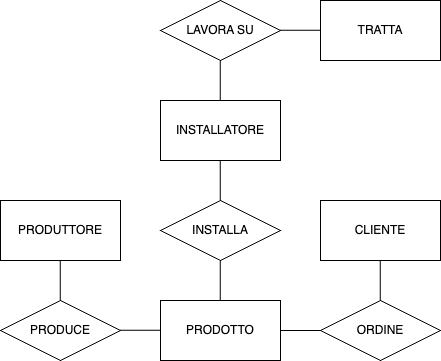
\includegraphics[width=10cm]{images/installatore.drawio.png}\\
    \caption{Schema scheletro della vista dell'Installatore}
\end{figure}

\subsection{Analisi requisiti e schema scheletro per l'Amministratore}

\begin{table}[H]
    \begin{tabular}{|l|l|l|l|}
    \hline
    \textbf{Termine} & Descrizione                                                                                             & Sinonimi          & Collegamenti                                                                                \\ \hline
    Amministratore   & Coordinatore generale                                                                                   & Manager           & \begin{tabular}[c]{@{}l@{}}Report, Sede, Team, \\ Cliente\end{tabular}                      \\ \hline
    Report           & Articolo riguardante Greenrail                                                                          & Notizia, Articolo & Amministratore                                                                              \\ \hline
    Sede             & \begin{tabular}[c]{@{}l@{}}Struttura in cui vengono costruiti\\ i prodotti Greenrail\end{tabular}       & Azienda           & Amministratore                                                                              \\ \hline
    Team             & Gruppo di persone                                                                                       & Squadra           & \begin{tabular}[c]{@{}l@{}}Amministratore, Produttori,\\ Installatori, Clienti\end{tabular} \\ \hline
    Cliente          & \begin{tabular}[c]{@{}l@{}}Enti o aziende, pubblici o privati, \\  nel settore ferroviario\end{tabular} & \begin{tabular}[c]{@{}l@{}}Azienda, \\ Ente\end{tabular} & Prodotto                                                                     \\ \hline
    Produttore       & Soggetto che realizza il prodotto                                                                       & -                 & Team, Installatori, Prodotto                                                                \\ \hline
    Installatore     & Soggetto che installa il prodotto                                                                       & -                 & Cliente, Prodotto, Team, Produttori                                                         \\ \hline
    Prodotto         & Articolo venduto da Greenrail                                                                           & Traversina        & \begin{tabular}[c]{@{}l@{}}Cliente, Installatore, Produttore,\\ Material\end{tabular}       \\ \hline
    Materiale        & \begin{tabular}[c]{@{}l@{}}Materiale di cui si compone un\\ prodotto\end{tabular}                       & -                 & Prodotto, Fornitore                                                                         \\ \hline
    Fornitore        & Soggetto che fornisce materiale                                                                         & Azienda           & Materiale                                                                                   \\ \hline
    \end{tabular}
    \caption{Glossario dei concetti dell'Amministratore}
\end{table}

\begin{figure}[H]
    \centering
    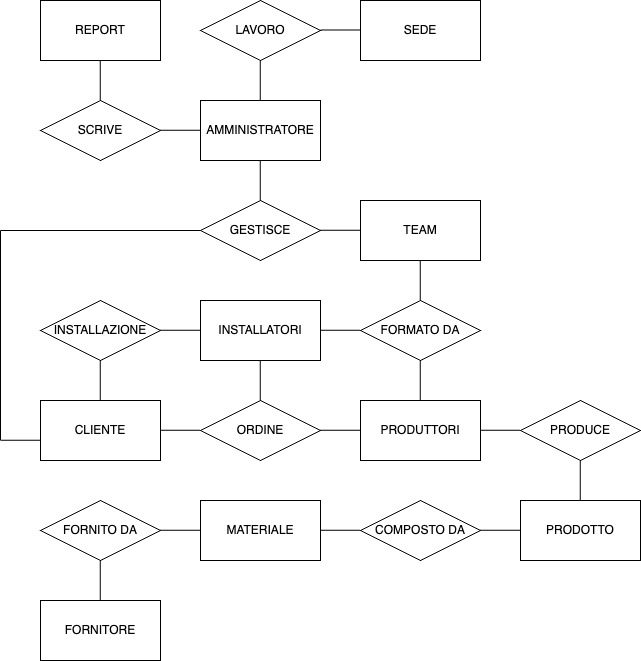
\includegraphics[width=13cm]{images/amministratore.drawio.png}\\
    \caption{Schema scheletro della vista dell'Amministratore}
\end{figure}

\section{Progettazione ed integrazione delle viste}
\subsection{Schemi E-R finali}
\subsubsection{Schema E-R del Cliente}

Nel passaggio dallo scheletro allo schema E-R finale, sono state apportate le modifiche:
\begin{enumerate}
    \item La relazione di Ordine diventa una entità, in quanto contiene informazioni aggiuntive rispetto a quelle del prodotto.
    \item L'entità Ordine viene storicizzata in Presente e Passato.
    \item Aggiunta l'istanza Modello da Prodotto per gestire i diversi modelli di traversina.
    \item L'entità Cliente generalizza i clienti Privato e Pubblico.
    \item Aggiunta l'entità Sede, generalizzazione di Sede Amministrativa e di Produzione in relazione con l'Amministratore.
\end{enumerate}


\subsubsection{Schema E-R del Produttore}
Nel passaggio dallo scheletro allo schema E-R finale, sono state apportate le modifiche:
\begin{enumerate}
    \item Modifica dell'errata entità Produttore in Sede che generalizza i tipi di Sede Amministrativa e di Produzione.
    \item Aggiunta entità Programma contente le informazioni relative alle attività del Produttore.
    \item La relazione di Ordine diventa una entità, in quanto contiene informazioni aggiuntive rispetto a quelle del prodotto.
    \item L'entità Ordine viene storicizzata in Presente e Passato.
    \item Aggiunta l'istanza Modello da Prodotto per gestire i diversi modelli di traversina.
    \item Aggiunta l'entità Componente, parte di un Modello, che generalizza un Componente Generico e Specifico.
\end{enumerate}




\subsubsection{Schema E-R dell'Installatore}
Nel passaggio dallo scheletro allo schema E-R finale, sono state apportate le modifiche:
\begin{enumerate}
    \item L'entità Tratta generalizza i tipi di Tratta Passeggeri e Merci.
    \item Come per la vista del Produttore, l'Installatore è parte di un Team.
    \item Aggiunta entità Programma contente le informazioni relative alle attività dell'Installatore.
    \item Aggiunta l'istanza Modello da Prodotto per gestire i diversi modelli di traversina.
    \item L'entità Ordine viene storicizzata in Presente e Passato.
    \item L'entità cliente generalizza i clienti Privato e Pubblico.
\end{enumerate}





\subsubsection{Schema E-R dell'Amministratore}
Nel passaggio dallo scheletro allo schema E-R finale, sono state apportate le modifiche:
\begin{enumerate}
    \item L'entità Sede generalizza i tipi di Sede Amministrativa e di Produzione.
    \item Aggiunta entità Dipendente che generalizza i tipi Amministratore e Operaio.
    \item L'entità Operaio generalizza a sua volta i tipi Produttore e Installatore.
    \item L'Amministratore gestisce Team e Ordine, non più Cliente.
    \item Aggiunta l'entità Tratta che generalizza i tipi di Tratta Passeggeri e Merci.
    \item L'entità Ordine viene storicizzata in Presente e Passato.
    \item L'entità Cliente generalizza i clienti Privato e Pubblico.
    \item Aggiunta entità Certificato che certifica la sostenibilità e sicurezza del prodotto.
    \item Aggiunta l'istanza Modello da Prodotto per gestire i diversi modelli di traversina.
    \item Aggiunta entità Componente, parte di un Modello, che generalizza un Componente Generico e Specifico.
\end{enumerate}




% \section{Methodology}
% This section has a subsection.
% \subsection{Subsection}
% This subsection contains \autoref{eq:1}.
% \begin{equation}
% \label{eq:1}
%     h(r) = \cfrac{Q}{2\pi T} \ln(\cfrac{r_i}{r_0})+h_0
% \end{equation}

% \section{Results}

% l

% \section{Discussion}

% As shown in previous studies, the proposed system has significant potential.

\newpage
\addcontentsline{toc}{section}{References}
\bibliographystyle{apalike}
\bibliography{ref}

% \newpage
% \appendix
% \section{Additional graphs and data}

\end{document}


%All other official TU Delft colours
\definecolor{donkerblauw}{RGB}{12, 35, 64}
\definecolor{turkoois}{RGB}{0, 184, 200}
\definecolor{blauw}{RGB}{0, 118, 194}
\definecolor{paars}{RGB}{111, 29, 119}
\definecolor{roze}{RGB}{239, 96, 163}
\definecolor{framboos}{RGB}{165, 0, 52}
\definecolor{rood}{RGB}{224, 60, 49}
\definecolor{oranje}{RGB}{237, 104, 66}
\definecolor{geel}{RGB}{255, 184, 28}
\definecolor{lichtgroen}{RGB}{108, 194, 74}
\definecolor{donkergroen}{RGB}{0, 155, 119}
%You can use these to change the hyperlink colour or the colour of the header or whatever. Glück Auf!
\end{itemize}hapter{Definizione e Analisi dei Requisiti}
